\documentclass{beamer}
\usepackage[utf8]{inputenc}
\usepackage{graphicx, epsfig}
\usepackage{amsmath,mathrsfs,amsfonts,amssymb}
\usepackage{floatflt}
\usepackage{epic,ecltree}
\usepackage{mathtext}
\usepackage{fancybox}
\usepackage{fancyhdr}
\usepackage{multirow}
\usepackage{enumerate}
\usepackage{epstopdf}
\usepackage{multicol}
\usepackage{algorithm}
\usepackage[noend]{algorithmic}
\usepackage{tikz}
\usepackage{blindtext}
\usetheme{default}%{Singapore}%{Warsaw}%{Warsaw}%{Darmstadt}
\usecolortheme{default}

\setbeamerfont{title}{size=\Huge}
\setbeamertemplate{footline}[page number]{}

\setbeamertemplate{section in toc}[sections numbered]


\makeatletter
\newcommand\HUGE{\@setfontsize\Huge{35}{40}}
\makeatother    

\setbeamerfont{title}{size=\HUGE}
\beamertemplatenavigationsymbolsempty

% latin bold lower
\newcommand{\ba}{\mathbf{a}} 
\newcommand{\bc}{\mathbf{c}} 
\newcommand{\be}{\mathbf{e}} 
\newcommand{\bh}{\mathbf{h}} 
\newcommand{\bp}{\mathbf{p}} 
\newcommand{\bt}{\mathbf{t}} 
\newcommand{\bs}{\mathbf{s}} 
\newcommand{\bu}{\mathbf{u}} 
\newcommand{\bv}{\mathbf{v}} 
\newcommand{\bw}{\mathbf{w}} 
\newcommand{\bx}{\mathbf{x}} 
\newcommand{\by}{\mathbf{y}} 
\newcommand{\bz}{\mathbf{z}} 

% latin bold upper
\newcommand{\bA}{\mathbf{A}} 
\newcommand{\bB}{\mathbf{B}} 
\newcommand{\bC}{\mathbf{C}} 
\newcommand{\bI}{\mathbf{I}} 
\newcommand{\bJ}{\mathbf{J}} 
\newcommand{\bL}{\mathbf{L}} 
\newcommand{\bM}{\mathbf{M}} 
\newcommand{\bP}{\mathbf{P}}
\newcommand{\bQ}{\mathbf{Q}} 
\newcommand{\bR}{\mathbf{R}} 
\newcommand{\bT}{\mathbf{T}} 
\newcommand{\bU}{\mathbf{U}} 
\newcommand{\bV}{\mathbf{V}} 
\newcommand{\bW}{\mathbf{W}} 
\newcommand{\bX}{\mathbf{X}} 
\newcommand{\bY}{\mathbf{Y}} 
\newcommand{\bZ}{\mathbf{Z}} 

% latin cal upper
\newcommand{\cF}{\mathcal{F}} 
\newcommand{\cG}{\mathcal{G}} 
\newcommand{\cI}{\mathcal{I}} 
\newcommand{\cL}{\mathcal{L}} 
\newcommand{\cM}{\mathcal{M}} 
\newcommand{\cN}{\mathcal{N}} 
\newcommand{\cP}{\mathcal{P}} 
\newcommand{\cS}{\mathcal{S}} 
\newcommand{\cT}{\mathcal{T}} 
\newcommand{\cW}{\mathcal{W}} 
\newcommand{\cX}{\mathcal{X}} 
\newcommand{\cZ}{\mathcal{Z}} 

% latin bb upper
\newcommand{\bbE}{\mathbb{E}} 
\newcommand{\bbI}{\mathbb{I}} 
\newcommand{\bbP}{\mathbb{P}} 
\newcommand{\bbR}{\mathbb{R}} 

% greek bold lower
\newcommand{\bepsilon}{\boldsymbol{\epsilon}} 
\newcommand{\btheta}{\boldsymbol{\theta}} 
\newcommand{\blambda}{\boldsymbol{\lambda}} 
\newcommand{\bpi}{\boldsymbol{\pi}} 
\newcommand{\bmu}{\boldsymbol{\mu}} 
\newcommand{\bsigma}{\boldsymbol{\sigma}} 
\newcommand{\bphi}{\boldsymbol{\phi}} 

% greek bold upper
\newcommand{\bSigma}{\boldsymbol{\Sigma}} 

\DeclareMathOperator*{\argmin}{arg\,min}
\DeclareMathOperator*{\argmax}{arg\,max}

\newcommand{\createdgmtitle}[1]{\title[\hbox to 56mm{Deep Generative Models  \hfill\insertframenumber\,/\,\inserttotalframenumber}]
	{\vspace{1cm} \\ \textbf{Deep Generative Models} \\ {\Huge Lecture #1}}
	\author{Roman Isachenko}
		\institute{
\includegraphics[width=0.7cm]{../utils/aimasterslogo} \LARGE{AI Masters}}
	\date{2024, Spring}
}

\usepackage{tikz}
\usetikzlibrary{arrows,shapes,positioning,shadows,trees}

\newcommand\myfootnote[1]{%
  \tikz[remember picture,overlay]
  \draw (current page.south west) +(1in + \oddsidemargin,0.5em)
  node[anchor=south west,inner sep=0pt]{\parbox{\textwidth}{%
      \rlap{\rule{10em}{0.4pt}}\raggedright\scriptsize \textit{#1}}};}

\newcommand\myfootnotewithlink[2]{%
  \tikz[remember picture,overlay]
  \draw (current page.south west) +(1in + \oddsidemargin,0.5em)
  node[anchor=south west,inner sep=0pt]{\parbox{\textwidth}{%
      \rlap{\rule{10em}{0.4pt}}\raggedright\scriptsize\href{#1}{\textit{#2}}}};}
      
\AtBeginSection[]
      {
      	\begin{frame}{Outline}
      		\tableofcontents[currentsection]
      	\end{frame}
      }
      \AtBeginSubsection[]{
      	\begin{frame}{Outline}
      		\tableofcontents[currentsection,currentsubsection]
      	\end{frame}
}
\createdgmtitle{4}
%--------------------------------------------------------------------------------
\begin{document}
%--------------------------------------------------------------------------------
\begin{frame}[noframenumbering,plain]
	%\thispagestyle{empty}
	\titlepage
\end{frame}
%=======
\begin{frame}{Recap of previous lecture}
	Let split $\bx$ and $\bz$ in two parts: 
	\[
	\bx = [\bx_1, \bx_2] = [\bx_{1:d}, \bx_{d+1:m}]; \quad \bz = [\bz_1, \bz_2] = [\bz_{1:d}, \bz_{d+1:m}].
	\]
	\vspace{-0.5cm}
	\begin{block}{Coupling layer}
		\vspace{-0.5cm}
		\[
		\begin{cases} {\color{violet}\bx_1} = {\color{teal}\bz_1}; \\ {\color{violet}\bx_2} = {\color{teal}\bz_2} \odot \bsigma_{\btheta}({\color{teal}\bz_1}) + \bmu_{\btheta}({\color{teal}\bz_1}).\end{cases}  
		\begin{cases} {\color{teal}\bz_1} ={\color{violet} \bx_1}; \\ {\color{teal}\bz_2} = \left({\color{violet}\bx_2} - \bmu_{\btheta}({\color{violet}\bx_1}) \right) \odot \frac{1}{\bsigma_{\btheta}({\color{violet}\bx_1})}.\end{cases}
		\]
		Estimating the density takes 1 pass, sampling takes 1 pass!
	\end{block}
	\begin{block}{Jacobian}
		\vspace{-0.3cm}
		\[
		\det \left( \frac{\partial \bz}{\partial \bx} \right) = \det 
		\begin{pmatrix}
			\bI_d & 0_{d \times m - d} \\
			\frac{\partial \bz_2}{\partial \bx_1} & \frac{\partial \bz_2}{\partial \bx_2}
		\end{pmatrix} = \prod_{j=1}^{m - d} \frac{1}{\sigma_j(\bx_1)}.
		\]
	\end{block}
	Coupling layer is a special case of autoregressive NF.
	
	\myfootnotewithlink{https://arxiv.org/abs/1605.08803}{Dinh L., Sohl-Dickstein J., Bengio S. Density estimation using Real NVP, 2016} 
\end{frame}
%=======
\begin{frame}{Recap of previous lecture}
	\begin{block}{Continuous-in-time dynamics}
		\vspace{-0.7cm}
		\begin{align*}
		   \frac{d \bz(t)}{dt} &= f_{\btheta}(\bz(t), t); \quad \text{with initial condition }\bz(t_0) = \bz_0. \\
		   \bz(t_1) &= \int^{t_1}_{t_0} f_{\btheta}(\bz(t), t) d t  + \bz_0 = \text{ODESolve}(\bz(t_0), f_{\btheta}, t_0,t_1).
		\end{align*}
		\vspace{-0.7cm}
	\end{block}	
	\begin{block}{Euler update step}
		\vspace{-0.6cm}
		\[
   \frac{\bz(t + \Delta t) - \bz(t)}{\Delta t} = f_{\btheta}(\bz(t), t) \,\, \Rightarrow \,\, \bz(t + \Delta t) = \bz(t) + \Delta t \cdot f_{\btheta}(\bz(t), t)
		\]
		\vspace{-0.7cm}
	\end{block}	
	\begin{block}{Theorem (Picard)}
		If $f$ is uniformly Lipschitz continuous in $\bz$ and continuous in $t$, then the ODE has a \textbf{unique} solution.
	\end{block}
		\vspace{-0.7cm}
		\begin{align*}
			\bx &= \bz(t_1) = \bz(t_0) + \int_{t_0}^{t_1} f_{\btheta}(\bz(t), t) dt \\
			\bz &= \bz(t_0) = \bz(t_1) + \int_{t_1}^{t_0} f_{\btheta}(\bz(t), t) dt
		\end{align*}
	\myfootnotewithlink{https://arxiv.org/abs/1806.07366}{Chen R. T. Q. et al. Neural Ordinary Differential Equations, 2018}   
\end{frame}
%=======
\begin{frame}{Recap of previous lecture}
	\begin{block}{Theorem (Kolmogorov-Fokker-Planck: special case)}
		If $f$ is uniformly Lipschitz continuous in $\bz$ and continuous in $t$, then
		\[
			\frac{d \log p(\bz(t), t)}{d t} = - \text{tr} \left( \frac{\partial f_{\btheta}(\bz(t), t)}{\partial \bz(t)} \right).
		\]
		\[
			\log p(\bz(t_1), t_1) = \log p(\bz(t_0), t_0) - \int_{t_0}^{t_1} \text{tr}  \left( \frac{\partial f_{\btheta}(\bz(t), t)}{\partial \bz(t)} \right) dt.
		\]
	\end{block}
	\begin{itemize}
		\item \textbf{Discrete-in-time NF}: evaluation of determinant of the Jacobian costs $O(m^3)$ (we need invertible $f$).
		\item \textbf{Continuous-in-time NF}: getting the trace of the Jacobian costs $O(m^2)$ (we need smooth $f$).
	\end{itemize}
	\begin{block}{Hutchinson's trace estimator}
		\vspace{-0.3cm}
		\[
  \log p(\bz(t_1)) = \log p(\bz(t_0)) - \mathbb{E}_{p(\bepsilon)} \int_{t_0}^{t_1} \left[ {\color{violet}\bepsilon^T \frac{\partial f}{\partial \bz}} \bepsilon \right] dt.
		\]
	\end{block}
	\myfootnotewithlink{https://arxiv.org/abs/1810.01367}{Grathwohl W. et al. FFJORD: Free-form Continuous Dynamics for Scalable Reversible Generative Models, 2018} 
\end{frame}
%=======
\begin{frame}{Recap of previous lecture}
	\begin{block}{Forward pass (Loss function)}
		\vspace{-0.3cm}
		\[
			\bz = \bx + \int_{t_1}^{t_0} f_{\btheta}(\bz(t), t) dt, \quad L(\bz) = \log p(\bz)
		\]
		\[
			L(\bz) = L\left( \bx + \int_{t_1}^{t_0} f_{\btheta}(\bz(t), t) dt \right) = L\bigl(\text{ODESolve}(\bx, f_{\btheta}, t_1, t_0) \bigr)
		\]
		\vspace{-0.5cm}
	\end{block}
	\begin{block}{Adjoint functions}
		\vspace{-0.4cm}
		\[
			\ba_{\bz}(t) = \frac{\partial L}{\partial \bz(t)}; \quad \ba_{\btheta}(t) = \frac{\partial L}{\partial \btheta(t)}.
		\]
		These functions show how the gradient of the loss depends on the hidden state~$\bz(t)$ and parameters $\btheta$.
		\vspace{-0.3cm}
	\end{block}

	\begin{block}{Theorem (Pontryagin)}
		\vspace{-0.6cm}
		\[
		\frac{d \ba_{\bz}(t)}{dt} = - \ba_{\bz}(t)^T \cdot \frac{\partial f_{\btheta}(\bz(t), t)}{\partial \bz}; \quad \frac{d \ba_{\btheta}(t)}{dt} = - \ba_{\bz}(t)^T \cdot \frac{\partial f_{\btheta}(\bz(t),  t)}{\partial \btheta}.
		\]
		\vspace{-0.7cm}
	\end{block}

	\myfootnotewithlink{https://arxiv.org/abs/1806.07366}{Chen R. T. Q. et al. Neural Ordinary Differential Equations, 2018}     
\end{frame}
%=======
\begin{frame}{Recap of previous lecture}
	\begin{block}{Forward pass}
		\vspace{-0.3cm}
		\[
		\bz = \bz(t_0) = \int^{t_1}_{t_0} f_{\btheta}(\bz(t), t) d t  + \bx \quad \Rightarrow \quad \text{ODE Solver}
		\]
		\vspace{-0.4cm}
	\end{block}
	\begin{block}{Backward pass}
		\vspace{-0.5cm}
		\begin{equation*}
			\left.
			{\footnotesize 
				\begin{aligned}
					\frac{\partial L}{\partial \btheta(t_1)} &= \ba_{\btheta}(t_1) =  - \int_{t_0}^{t_1} \ba_{\bz}(t)^T \frac{\partial f_{\btheta}(\bz(t), t)}{\partial \btheta(t)} dt + 0 \\
					\frac{\partial L}{\partial \bz(t_1)} &= \ba_{\bz}(t_1) =  - \int_{t_0}^{t_1} \ba_{\bz}(t)^T \frac{\partial f_{\btheta}(\bz(t), t)}{\partial \bz(t)} dt + \frac{\partial L}{\partial \bz(t_0)} \\
					\bz(t_1) &= - \int^{t_0}_{t_1} f_{\btheta}(\bz(t), t) d t  + \bz_0.
				\end{aligned}
			}
			\right\rbrace
			\Rightarrow
			\text{ODE Solver}
		\end{equation*}
		\vspace{-0.4cm} 
	\end{block}
	\textbf{Note:} These scary formulas are the standard backprop in the discrete case.
	\myfootnotewithlink{https://arxiv.org/abs/1806.07366}{Chen R. T. Q. et al. Neural Ordinary Differential Equations, 2018}   
\end{frame}
%=======
\begin{frame}{Outline}
	\tableofcontents
\end{frame}
%=======
\section{Latent variable models (LVM)}
%=======
\begin{frame}{Generative models zoo}
	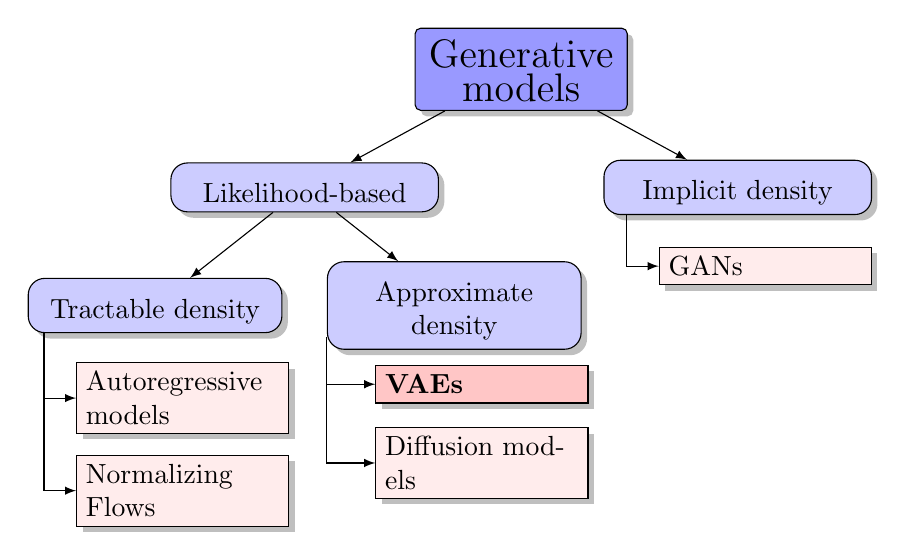
\begin{tikzpicture}[
	 	basic/.style  = {draw, text width=2cm, drop shadow, rectangle},
	 	root/.style   = {basic, rounded corners=2pt, thin, text height=1.1em, text width=7em, align=center, fill=blue!40},
	 	level 1/.style={sibling distance=55mm},
	 	level 2/.style = {basic, rounded corners=6pt, thin, align=center, fill=blue!20, text height=1.1em, text width=9em, sibling distance=38mm},
	 	level 3/.style = {basic, rounded corners=6pt, thin,align=center, fill=blue!20, text width=8.5em},
	 	level 4/.style = {basic, thin, align=left, fill=pink!30, text width=7em},
	 	level 5/.style = {basic, thin, align=left, fill=pink!90, text width=7em},
		edge from parent/.style={->,draw},
		>=latex]
		
		% root of the the initial tree, level 1
		\node[root] {\Large Generative models}
		% The first level, as children of the initial tree
		child {node[level 2] (c1) {Likelihood-based}
			child {node[level 3] (c11) {Tractable density}}
			child {node[level 3] (c12) {Approximate density}}
		}
		child {node[level 2] (c2) {Implicit density}};
		
		% The second level, relatively positioned nodes
		\begin{scope}[every node/.style={level 5}]
		\node [below of = c12, xshift=10pt] (c121) {\textbf{VAEs}};
		\end{scope}
	
		% The second level, relatively positioned nodes
		\begin{scope}[every node/.style={level 4}]
			\node [below of = c11, yshift=-5pt, xshift=10pt] (c111) {Autoregressive models};
			\node [below of = c111, yshift=-5pt] (c112) {Normalizing Flows};
			
			\node [below of = c121] (c122) {Diffusion models};
			
			\node [below of = c2, xshift=10pt] (c21) {GANs};
		\end{scope}
	
		
		% lines from each level 1 node to every one of its "children"
		\foreach \value in {1,2}
		\draw[->] (c11.194) |- (c11\value.west);
		
		\foreach \value in {1,2}
		\draw[->] (c12.194) |- (c12\value.west);
		
		\draw[->] (c2.194) |- (c21.west);
		
	\end{tikzpicture}
\end{frame}
%=======
\begin{frame}{Bayesian framework}
	\begin{block}{Bayes theorem}
		\[
			p(\bt | \bx) = \frac{p(\bx | \bt) p(\bt)}{p(\bx)} = \frac{p(\bx | \bt) p(\bt)}{\int p(\bx | \bt) p(\bt) d \bt} 
		\]
		\begin{itemize}
			\item $\bx$ -- observed variables, $\bt$ -- unobserved variables (latent variables/parameters);
			\item $p(\bx | \bt)$ -- likelihood;
			\item $p(\bx) = \int p(\bx | \bt) p(\bt) d \bt$ -- evidence;
			\item $p(\bt)$ -- prior distribution, $p(\bt | \bx)$ -- posterior distribution.
		\end{itemize}
	\end{block}
	\begin{block}{Meaning}
		We have unobserved variables $\bt$ and some prior knowledge about them $p(\bt)$. Then, the data $\bx$ has been observed. 
		Posterior distribution $p(\bt | \bx)$ summarizes the knowledge after the observations.
	\end{block}
\end{frame}
%=======
\begin{frame}{Bayesian framework}
	Let consider the case, where the unobserved variables $\bt$ is our model parameters $\btheta$.
	\begin{itemize}
		\item $\bX = \{\bx_i\}_{i=1}^n$ -- observed samples;
		\item $p(\btheta)$ -- prior parameters distribution (we treat model parameters $\btheta$ as random variables).
	\end{itemize}
	\begin{block}{Posterior distribution}
		\[
			p(\btheta | \bX) = \frac{p(\bX | \btheta) p(\btheta)}{p(\bX)} = \frac{p(\bX | \btheta) p(\btheta)}{\int p(\bX | \btheta) p(\btheta) d \btheta} 
		\]
		\vspace{-0.2cm}
	\end{block}
	If evidence $p(\bX)$ is intractable (due to multidimensional integration), we can't get posterior distribution and perform the exact inference.
    \begin{block}{Maximum a posteriori (MAP) estimation}
    \vspace{-0.2cm}
    \[
        \btheta^* = \argmax_{\btheta} p(\btheta | \bX) = \argmax_{\btheta} \bigl(\log p(\bX | \btheta) + \log p(\btheta) \bigr)
    \]
    \end{block}
\end{frame}
%=======
\begin{frame}{Latent variable models (LVM)}
	\begin{block}{MLE problem}
		\vspace{-0.5cm}
		\[
		\btheta^* = \argmax_{\btheta} p(\bX | \btheta) = \argmax_{\btheta} \prod_{i=1}^n p(\bx_i | \btheta) = \argmax_{\btheta} \sum_{i=1}^n \log p(\bx_i | \btheta).
		\]
		\vspace{-0.5cm}
	\end{block}
	The distribution $p(\bx | \btheta)$ could be very complex and intractable (as well as real distribution $\pi(\bx)$).
	\begin{block}{Extended probabilistic model}
		Introduce latent variable $\bz$ for each sample $\bx$
		\[
		p(\bx, \bz | \btheta) = p(\bx | \bz, \btheta) p(\bz); \quad 
		\log p(\bx, \bz | \btheta) = \log p(\bx | \bz, \btheta) + \log p(\bz).
		\]
		\[
		p(\bx | \btheta) = \int p(\bx, \bz | \btheta) d\bz = \int p(\bx | \bz, \btheta) p(\bz) d\bz.
		\]
	\end{block}
	\vspace{-0.3cm}
	\begin{block}{Motivation}
		The distributions $p(\bx | \bz, \btheta)$ and $p(\bz)$ could be quite simple.
	\end{block}
\end{frame}
%=======
\begin{frame}{Latent variable models (LVM)}
	\[
	\log p(\bx | \btheta) = \log \int p(\bx | \bz, \btheta) p(\bz) d\bz \rightarrow \max_{\btheta}
	\]
	\vspace{-0.6cm}
	\begin{block}{Examples}
		\begin{minipage}[t]{0.45\columnwidth}
			\textit{Mixture of gaussians} \\
			\vspace{-0.5cm}
			\begin{figure}
				\centering
				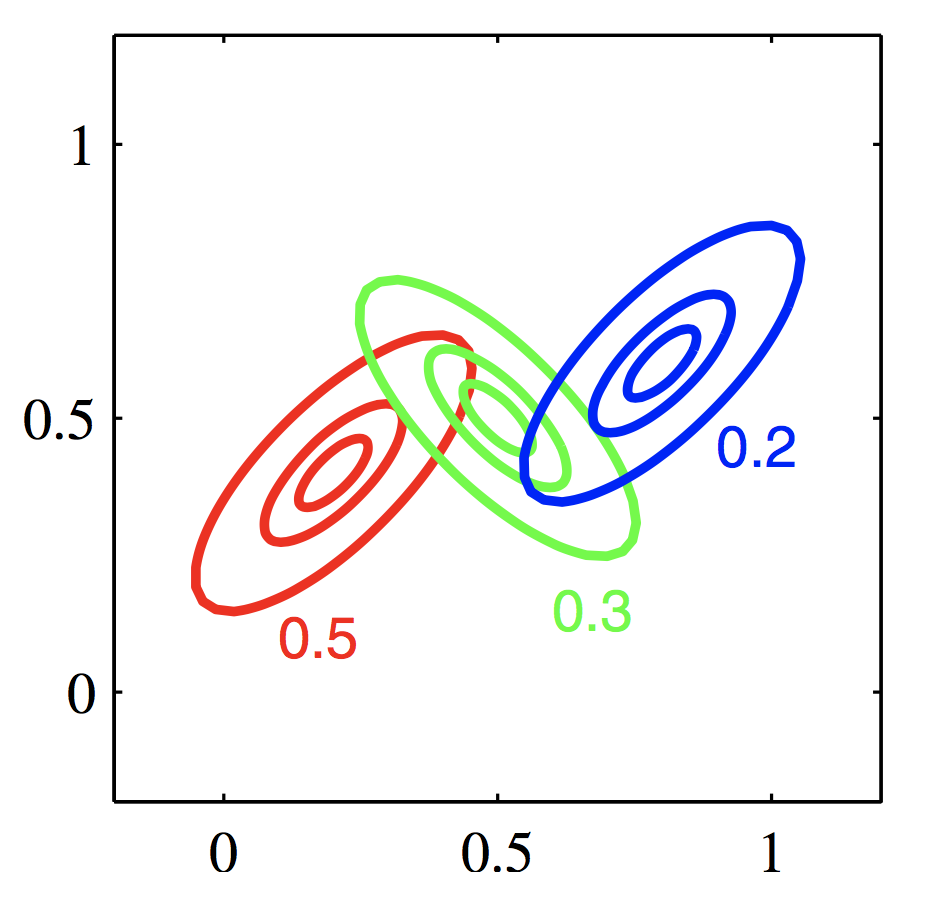
\includegraphics[width=0.75\linewidth]{figs/mixture_of_gaussians}
			\end{figure}
			\vspace{-0.5cm}
			\begin{itemize}
				\item $p(\bx | z, \btheta) = \cN(\bx | \bmu_z, \bSigma_z)$
				\item $p(z) = \text{Categorical}(\bpi)$
			\end{itemize}
		\end{minipage}%
		\begin{minipage}[t]{0.53\columnwidth}
			\textit{PCA model} \\
			\vspace{-0.5cm}
			\begin{figure}
				\centering
				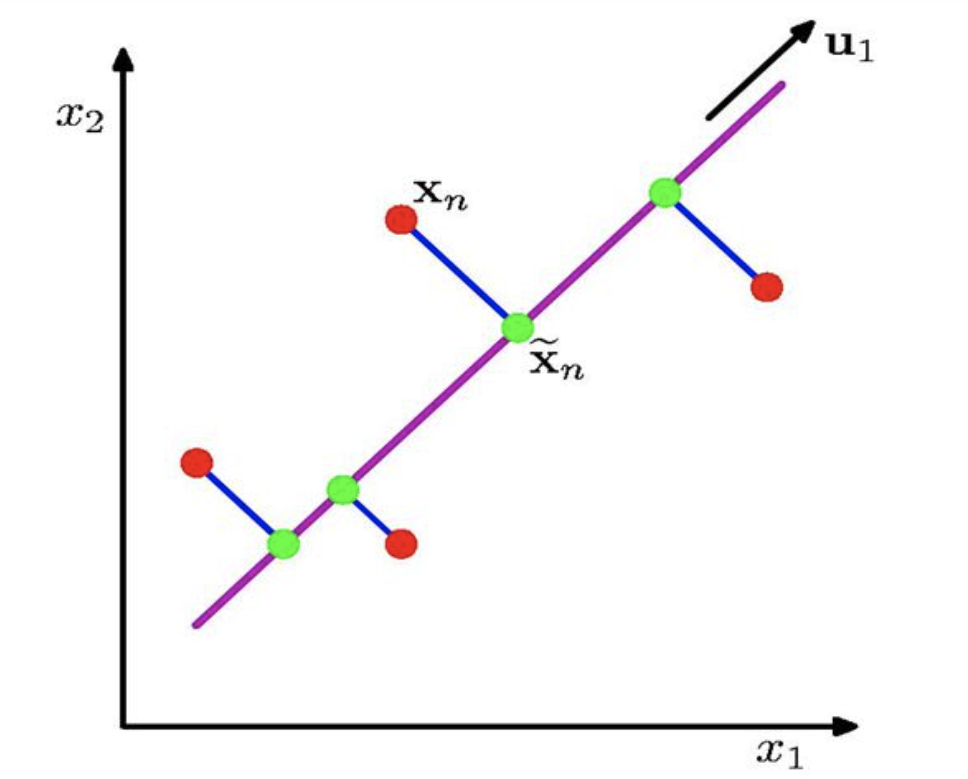
\includegraphics[width=.7\linewidth]{figs/pca}
			\end{figure}
			\vspace{-0.3cm}
			\begin{itemize}
				\item $p(\bx | \bz, \btheta) = \cN(\bx | \bW \bz + \bmu, \sigma^2 \bI)$
				\item $p(\bz) = \cN(\bz | 0, \bI)$
			\end{itemize}
		\end{minipage}
	\end{block}
	\myfootnote{Bishop\,C. Pattern Recognition and Machine Learning, 2006}
\end{frame}
%=======
\begin{frame}{Latent variable models (LVM)}
	\[
	\log p(\bx | \btheta) = \log \int p(\bx | \bz, \btheta) p(\bz) d\bz \rightarrow \max_{\btheta}
	\]
	\textbf{PCA} projects original data $\bX$ onto a low dimensional latent space while maximizing the variance of the projected data. 
	\begin{figure}
		\centering
		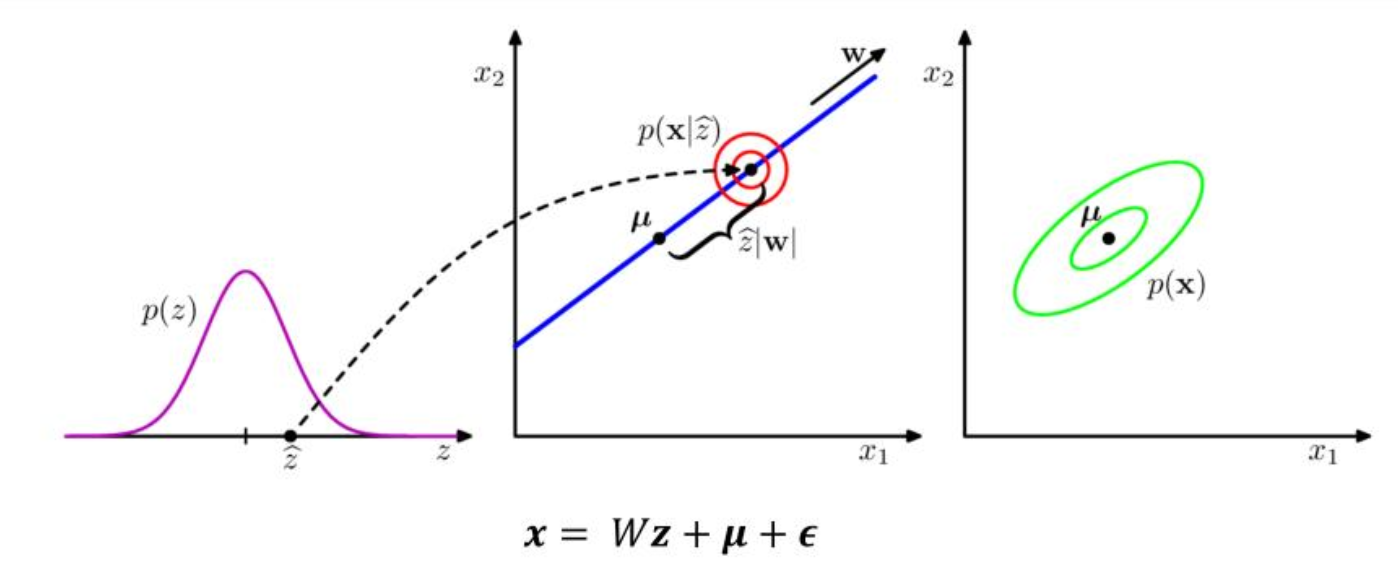
\includegraphics[width=.7\linewidth]{figs/bayesian_pca}
	\end{figure}
	\vspace{-0.5cm}
	\begin{itemize}
		\item $p(\bx | \bz, \btheta) = \cN(\bx | \bW \bz + \bmu, \sigma^2 \bI)$
		\item $p(\bz) = \cN(\bz | 0, \bI)$
		\item $p(\bx) = \cN(\bx | \bmu, \bW \bW^T + \sigma^2 \bI)$
		\item $p(\bz | \bx) = \cN \bigl(\bM^{-1} \bW^T (\bx - \bmu), \sigma^2 \bM\bigr)$, where $\bM = \bW \bW^T + \sigma^2 \bI$
	\end{itemize}
\end{frame}
%=======
\begin{frame}{Maximum likelihood estimation for LVM}
	\begin{block}{MLE for extended problem}
		\vspace{-0.7cm}
		\begin{multline*}
			\vspace{-0.5cm}
			\btheta^* = \argmax_{\btheta} p(\bX, \bZ | \btheta) = \argmax_{\btheta} \prod_{i=1}^n p(\bx_i, \bz_i | \btheta) = \\ = \argmax_{\btheta} \sum_{i=1}^n \log p(\bx_i, \bz_i | \btheta).
		\end{multline*}
		\vspace{-0.5cm}
	\end{block}
	However, $\bZ$ is unknown.
	\begin{block}{MLE for original problem}
		\vspace{-0.7cm}
		\begin{multline*}
			\btheta^* = \argmax_{\btheta} \log p(\bX| \btheta) = \argmax_{\btheta} \sum_{i=1}^n \log p(\bx_i | \btheta) = \\ =  \argmax_{\btheta}  \sum_{i=1}^n \log \int p(\bx_i, \bz_i | \btheta) d \bz_i = \\ = \argmax_{\btheta} \log \sum_{i=1}^n \int p(\bx_i| \bz_i, \btheta) p(\bz_i) d\bz_i.
		\end{multline*}
	\end{block}
	
\end{frame}
%=======
\begin{frame}{Naive approach}
	\begin{figure}
		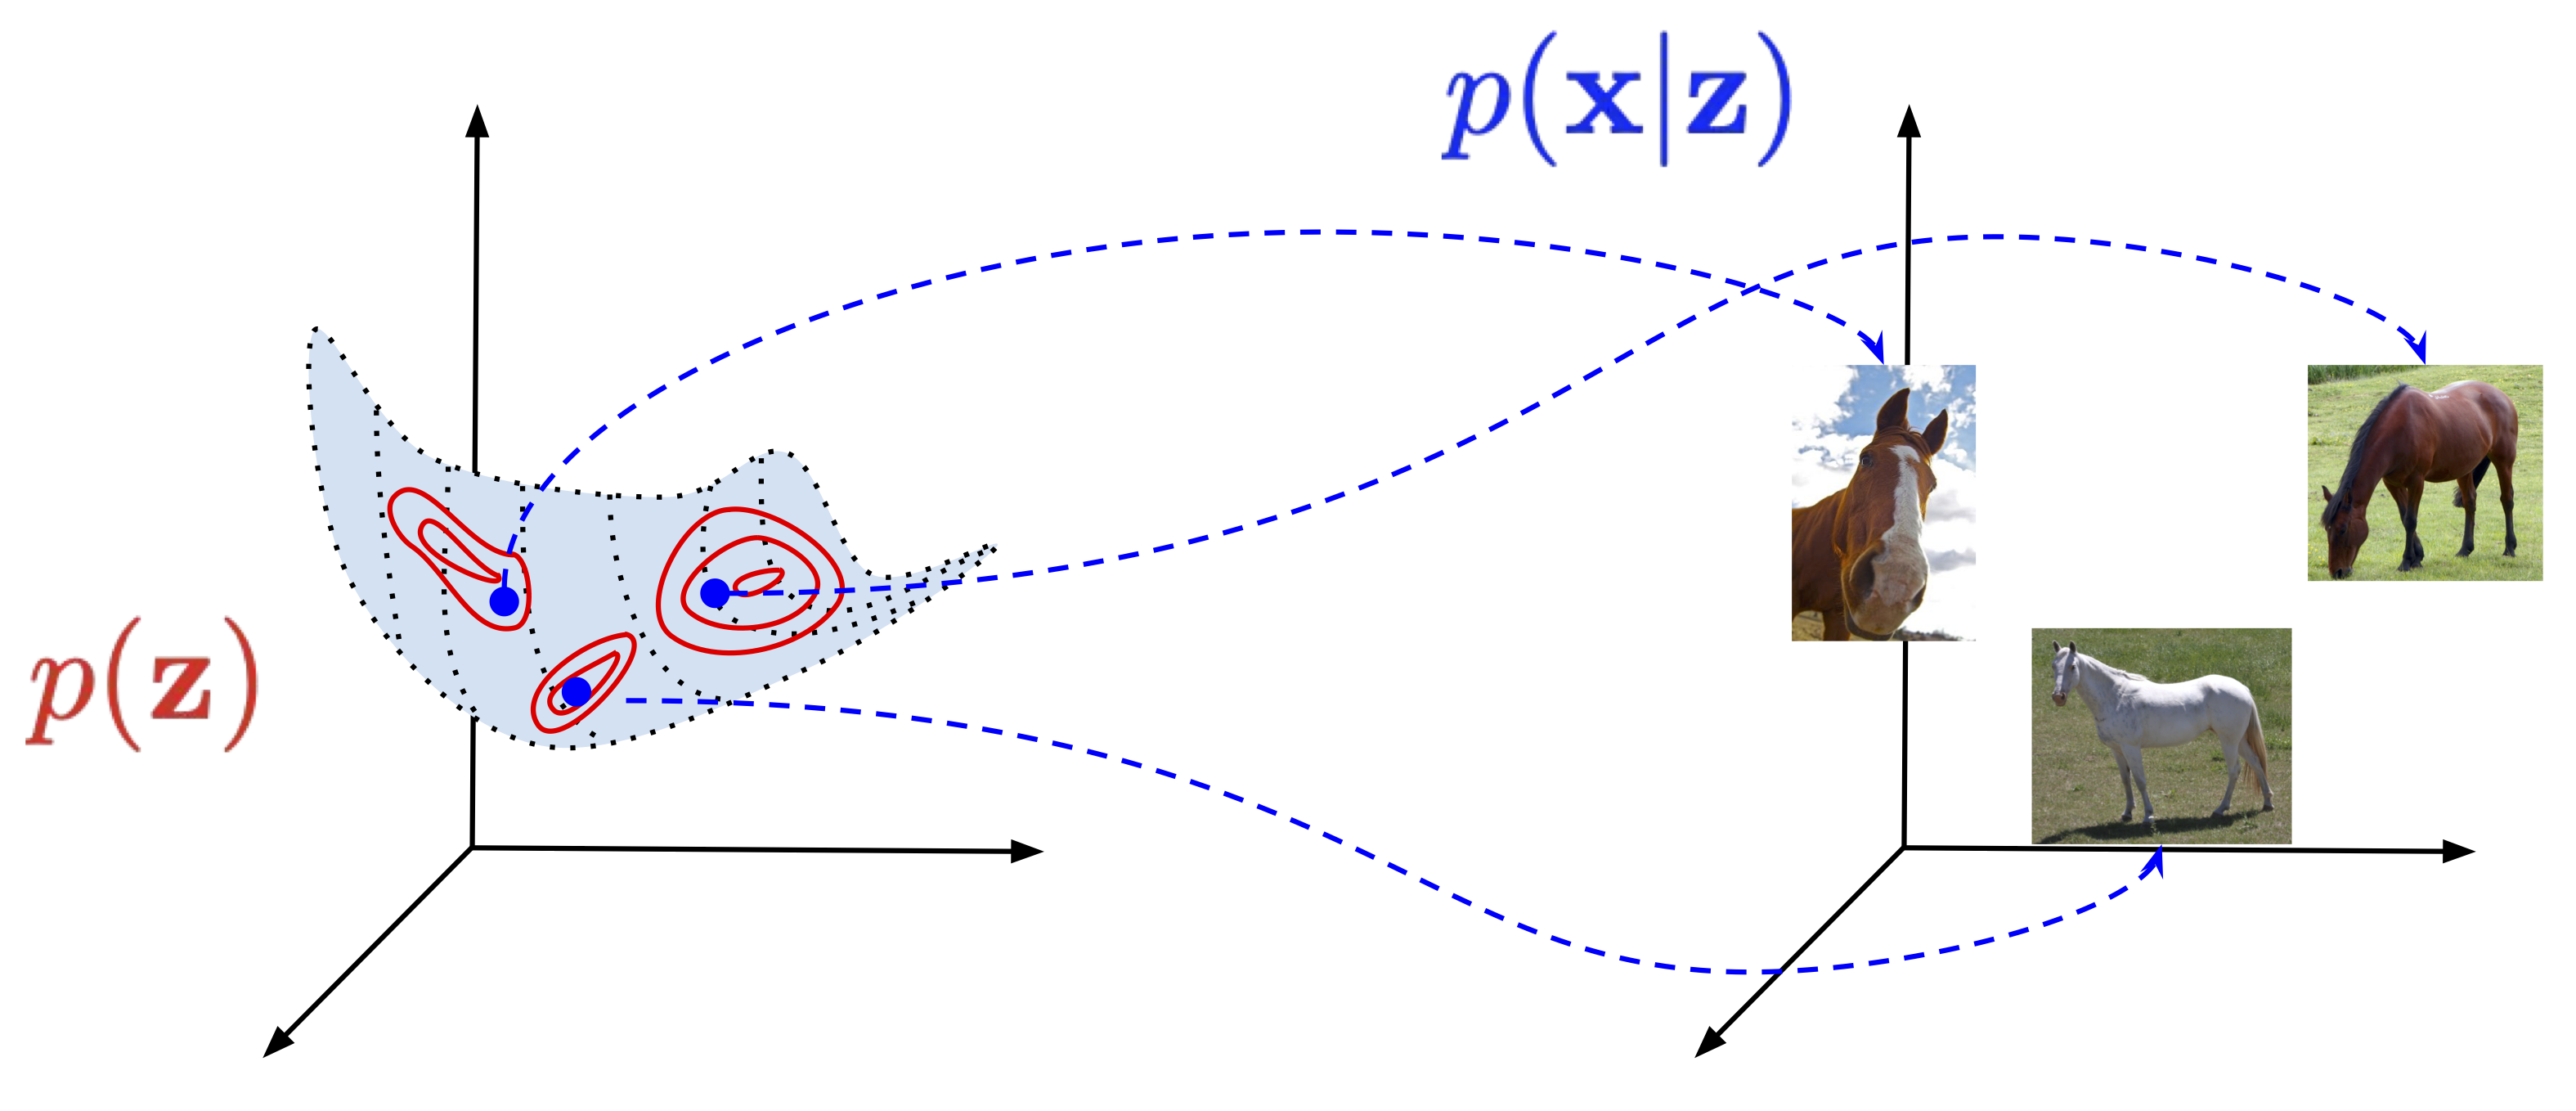
\includegraphics[width=.75\linewidth]{figs/lvm_diagram}
	\end{figure}
	\begin{block}{Monte-Carlo estimation}
		\vspace{-0.7cm}
		\[
			p(\bx | \btheta) = \int p(\bx | \bz, \btheta) p(\bz) d\bz = \bbE_{p(\bz)} p(\bx | \bz, \btheta) \approx \frac{1}{K} \sum_{k=1}^{K} p(\bx | \bz_k, \btheta),
		\]
		\vspace{-0.5cm} \\
		where $\bz_k \sim p(\bz)$. \\
		\textbf{Challenge:} to cover the space properly, the number of samples grows exponentially with respect to dimensionality of $\bz$. 
	\end{block}
	\myfootnotewithlink{https://jmtomczak.github.io/blog/4/4\_VAE.html}{image credit: https://jmtomczak.github.io/blog/4/4\_VAE.html}
\end{frame}
%=======
\section{Variational lower bound (ELBO)}
%=======
\begin{frame}{Variational lower bound (ELBO)}
	\begin{block}{Derivation 1 (inequality)}
		\vspace{-0.7cm}
		\begin{multline*}
			\log p(\bx| \btheta) 
			= \log \int p(\bx, \bz | \btheta) d\bz = \log \int \frac{q(\bz)}{q(\bz)} p(\bx, \bz | \btheta) d\bz = \\
			= \log \bbE_{q} \left[\frac{p(\bx, \bz| \btheta)}{q(\bz)} \right] \geq \bbE_{q} \log \frac{p(\bx, \bz| \btheta)}{q(\bz)} =  \cL(q, \btheta)
		\end{multline*}
		\vspace{-0.7cm}
	\end{block}
	\begin{block}{Derivation 2 (equality)}
		\vspace{-0.7cm}
		\begin{multline*}
			\mathcal{L} (q, \btheta) = \int q(\bz) \log \frac{p(\bx, \bz | \btheta)}{q(\bz)}d\bz = 
			\int q(\bz) \log \frac{p(\bz|\bx, \btheta)p(\bx| \btheta)}{q(\bz)}d\bz = \\
			= \int q(\bz) \log p(\bx| \btheta) d\bz + \int q(\bz) \log \frac{p(\bz|\bx, \btheta)}{q(\bz)}d\bz = \\
			= \log p(\bx| \btheta) - KL(q(\bz) || p(\bz|\bx, \btheta))
		\end{multline*}
	\end{block}
	\vspace{-0.7cm}
	\begin{block}{Variational decomposition}
		\[
			\log p(\bx| \btheta) = \mathcal{L} (q, \btheta) + KL(q(\bz) || p(\bz|\bx, \btheta)) \geq \mathcal{L} (q, \btheta).
		\]
	\end{block}
\end{frame}
%=======
\begin{frame}{Variational lower bound (ELBO)}
	\vspace{-0.3cm}
	\begin{align*}
		\mathcal{L} (q, \btheta) &= \int q(\bz) \log \frac{\color{violet}p(\bx, \bz | \btheta)}{\color{teal}q(\bz)}d\bz = \\ 
		&= \int q(\bz) \log {\color{violet}p(\bx | \bz, \btheta)} d\bz + \int q(\bz) \log \frac{\color{violet}p(\bz)}{\color{teal}q(\bz)}d\bz \\ 
		&= \mathbb{E}_{q} \log p(\bx | \bz, \btheta) - KL (q(\bz) || p(\bz))
	\end{align*}
	\vspace{-0.5cm}
	\begin{block}{Log-likelihood decomposition}
		\vspace{-0.8cm}
		\begin{multline*}
			\log p(\bx| \btheta) = {\color{olive}\mathcal{L} (q, \btheta)} + KL(q(\bz) || p(\bz|\bx, \btheta)) \\ = {\color{olive}\mathbb{E}_{q} \log p(\bx | \bz, \btheta) - KL (q(\bz) || p(\bz))} + KL(q(\bz) || p(\bz|\bx, \btheta)).
		\end{multline*}
		\vspace{-0.7cm}
	\end{block}
	\begin{itemize}
		\item Instead of maximizing incomplete likelihood, maximize ELBO
		\[
		\max_{\btheta} p(\bx | \btheta) \quad \rightarrow \quad \max_{q, \btheta} \mathcal{L} (q, \btheta)
		\]
		\item Maximization of ELBO by \textbf{variational} distribution $q$ is equivalent to minimization of KL
		\[
		\argmax_q \mathcal{L} (q, \btheta) \equiv \argmin_q KL(q(\bz) || p(\bz|\bx, \btheta)).
		\]
	\end{itemize}
\end{frame}
%=======
\section{EM-algorithm, amortized inference}
%=======
\begin{frame}{EM-algorithm}
	\vspace{-0.5cm}
	\begin{multline*}
		\mathcal{L} (q, \btheta)  =  \mathbb{E}_{q} \log p(\bx | \bz, \btheta) - KL (q(\bz) || p(\bz)) = \\ = \bbE_q \left[ \log p(\bx | \bz, \btheta) - \log \frac{q(\bz)}{p(\bz)} \right]d\bz \rightarrow \max_{q, \btheta}.
	\end{multline*}
	\vspace{-0.5cm}
	\begin{block}{Block-coordinate optimization}
		\begin{itemize}
			\item Initialize $\btheta^*$;
			\item \textbf{E-step} ($\mathcal{L} (q, \btheta) \rightarrow \max_q$)
			\vspace{-0.2cm}
			\begin{multline*}
				q^*(\bz) = \argmax_q \mathcal{L} (q, \btheta^*) = \\
				= \argmin_q KL(q(\bz) || p(\bz | \bx, \btheta^*)) = p(\bz| \bx, \btheta^*);
			\end{multline*}
			\item \textbf{M-step} ($\mathcal{L} (q, \btheta) \rightarrow \max_{\btheta}$)
			\vspace{-0.2cm}
			\[
			\btheta^* = \argmax_{\btheta} \mathcal{L} (q^*, \btheta);
			\]
			\vspace{-0.2cm}
			\item Repeat E-step and M-step until convergence.
		\end{itemize}
	\end{block}
\end{frame}
%=======
\begin{frame}{EM-algorithm illustration}
	
	\begin{minipage}[t]{0.45\columnwidth}
		\begin{figure}
			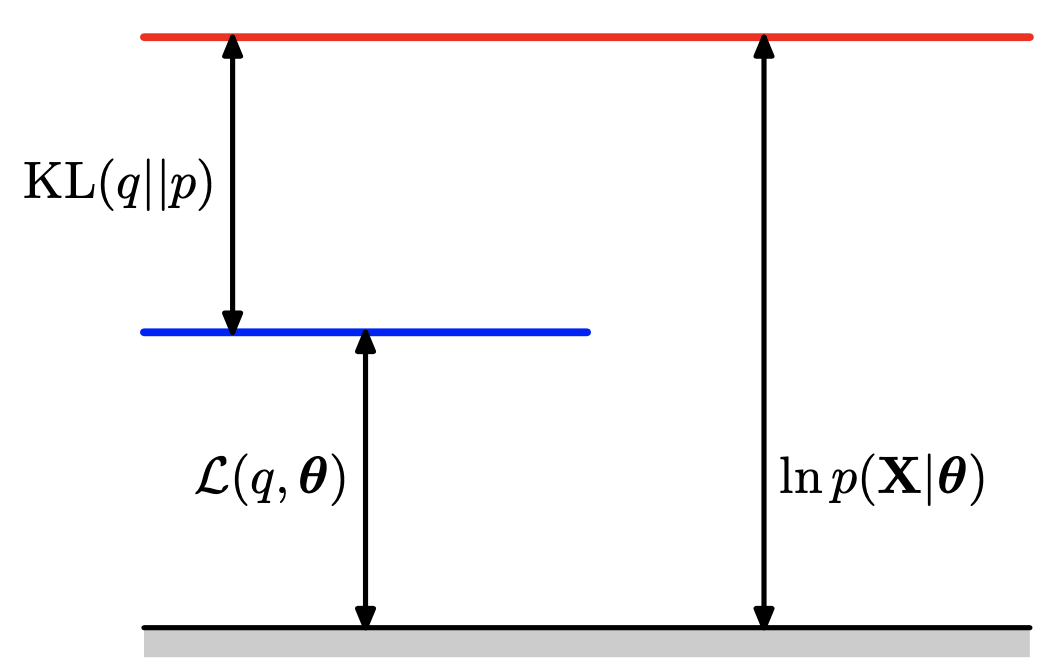
\includegraphics[width=0.9\linewidth]{figs/em_bishop1}
		\end{figure}
	\end{minipage}%
	\begin{minipage}[t]{0.55\columnwidth}
		\begin{figure}
			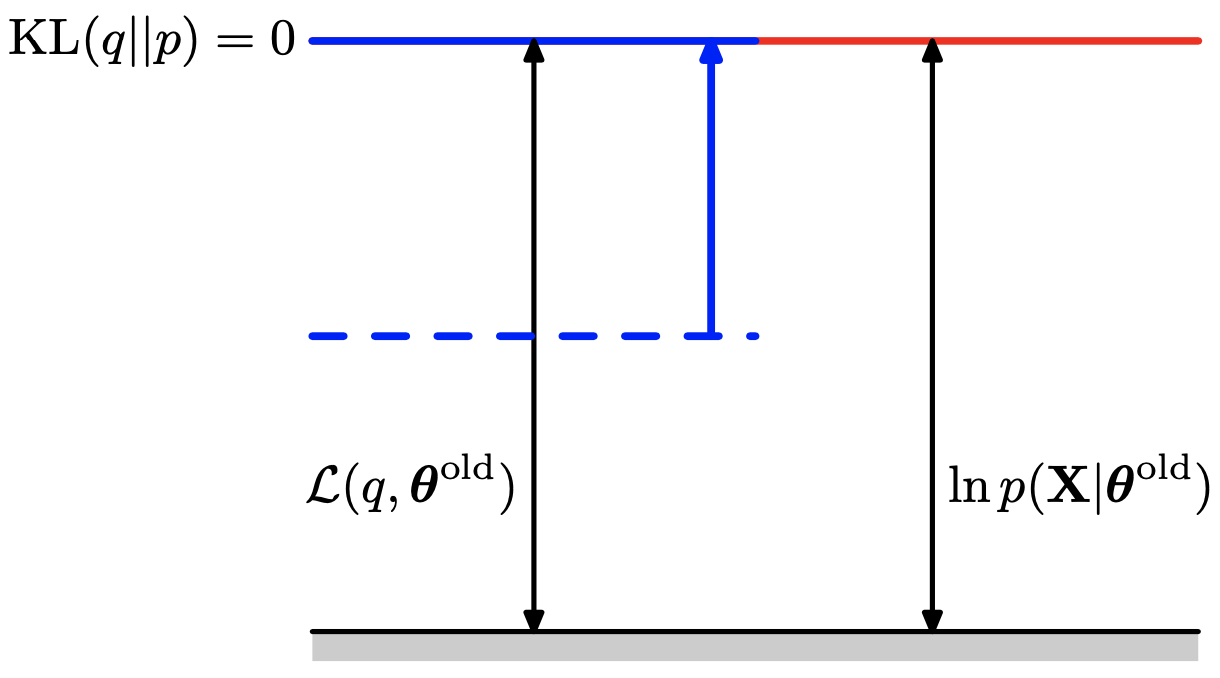
\includegraphics[width=0.85\linewidth]{figs/em_bishop2}
		\end{figure}
	\end{minipage}
	\begin{figure}
		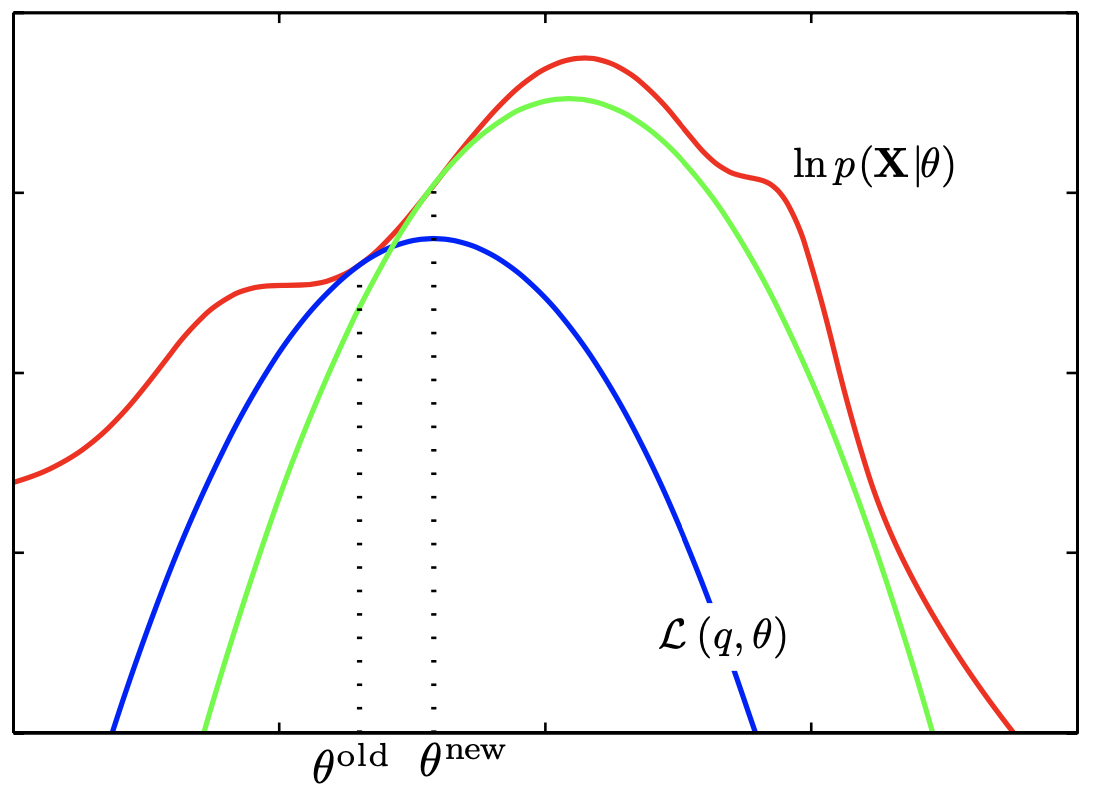
\includegraphics[width=.55\linewidth]{figs/em_bishop3}
	\end{figure}
	
	\myfootnote{Bishop\,C. Pattern Recognition and Machine Learning, 2006}
\end{frame}
%=======
\begin{frame}{Amortized variational inference}
	\begin{block}{E-step}
		\vspace{-0.3cm}
		\[
		q(\bz) = \argmax_q \mathcal{L} (q, \btheta^*) = \argmin_q KL(q || p) =
		p(\bz| \bx, \btheta^*).
		\]
		\vspace{-0.3cm}
		\begin{itemize}
			\item $q(\bz)$ approximates true posterior distribution $p(\bz| \bx, \btheta^*)$, that is why it is called \textbf{variational posterior};
			\item $p(\bz| \bx, \btheta^*)$ could be \textbf{intractable};
			\item $q(\bz)$ is different for each object $\bx$.
		\end{itemize}
		\vspace{-0.3cm}
	\end{block}
	\begin{block}{Idea}
		Restrict a family of all possible distributions $q(\bz)$ to a parametric class $q(\bz|\bx, \bphi)$ conditioned on samples $\bx$ with parameters $\bphi$.
	\end{block}
	
	\textbf{Variational Bayes}
	\begin{itemize}
		\item E-step
		\[
			\bphi_k = \bphi_{k-1} + \left.\eta \nabla_{\bphi} \mathcal{L}(\bphi, \btheta_{k-1})\right|_{\bphi=\bphi_{k-1}}
		\]
		\item M-step
		\[
			\btheta_k = \btheta_{k-1} + \left.\eta \nabla_{\btheta} \mathcal{L}(\bphi_k, \btheta)\right|_{\btheta=\btheta_{k-1}}
		\]
	\end{itemize}
\end{frame}
%=======
\begin{frame}{Variational EM illustration}
	\begin{itemize}
		\item E-step
		\[
			\bphi_k = \bphi_{k-1} + \left.\eta \nabla_{\bphi} \mathcal{L}(\bphi, \btheta_{k-1})\right|_{\bphi=\bphi_{k-1}}
		\]
		\item M-step
		\[
			\btheta_k = \btheta_{k-1} + \left.\eta \nabla_{\btheta} \mathcal{L}(\bphi_k, \btheta)\right|_{\btheta=\btheta_{k-1}}
		\]
	\end{itemize}
	\begin{figure}
		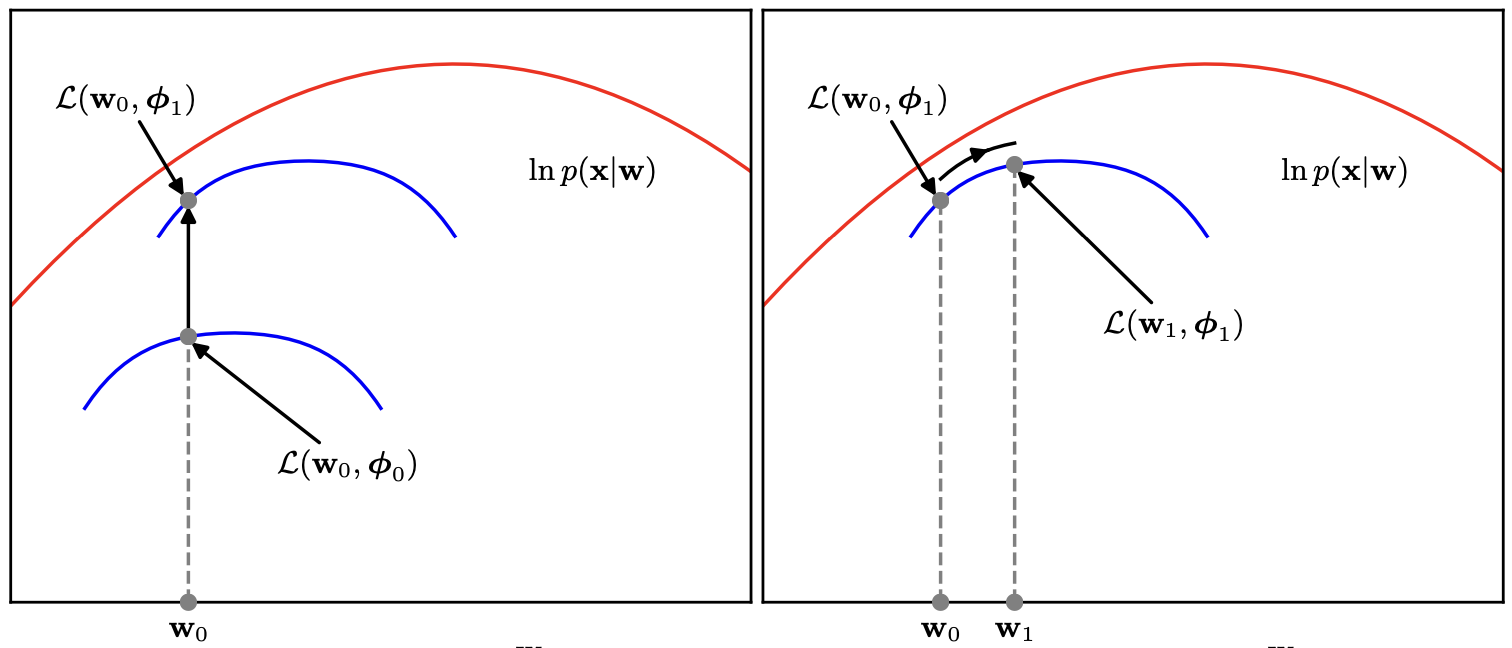
\includegraphics[width=\linewidth]{figs/em_bishop4}
	\end{figure}
		
	\myfootnote{Bishop\,C. Deep Learning: Foundations and Concepts, 2024}
\end{frame}
%=======
\begin{frame}{Variational EM-algorithm}
	\begin{block}{ELBO}
		\vspace{-0.5cm}
		\[
		\log p(\bx| \btheta) = \mathcal{L} (\bphi, \btheta) + KL(q(\bz | \bx, \bphi) || p(\bz|\bx, \btheta)) \geq \mathcal{L} (\bphi, \btheta).
		\]
		\vspace{-0.5cm}
	\end{block}
	\begin{itemize}
		\item \textbf{E-step}
		\[
		\bphi_k = \bphi_{k-1} + \left.\eta \nabla_{\bphi} \mathcal{L}(\bphi, \btheta_{k-1})\right|_{\bphi=\bphi_{k-1}},
		\]
		where $\bphi$~-- parameters of variational posterior distribution $q(\bz | \bx, \bphi)$.
		\item \textbf{M-step}
		\[
		\btheta_k = \btheta_{k-1} + \left.\eta \nabla_{\btheta} \mathcal{L}(\bphi_k, \btheta)\right|_{\btheta=\btheta_{k-1}},
		\]
		where $\btheta$~-- parameters of the generative distribution $p(\bx | \bz, \btheta)$.
	\end{itemize}
	Now all we have to do is to obtain two gradients $\nabla_{\bphi} \mathcal{L}(\bphi, \btheta)$, $\nabla_{\btheta} \mathcal{L}(\bphi, \btheta)$.  \\
	\textbf{Challenge:} Number of samples $n$ could be huge (we heed to derive unbiased stochastic gradients).
\end{frame}
%=======
\begin{frame}{Summary}
	\begin{itemize}
		\item Bayesian framework is a generalization of most common machine learning tasks.
		\vfill
		\item LVM introduces latent representation of observed samples to make model more interpretable.
		\vfill
		\item LVM maximizes variational evidence lower bound (ELBO) to find MLE for the parameters.
		\vfill
		\item The general variational EM algorithm maximizes ELBO objective for LVM model to find MLE for parameters $\btheta$.
	\end{itemize}
\end{frame}
%=======
\end{document} 